% -*- root: ../thesis.tex -*-
%!TEX root = ../thesis.tex
% ******************************* Thesis Chapter 2 ****************************


% ----------------------- paths to graphics ------------------------

% change according to folder and file names
\graphicspath{{2_background/figures/}}
% ----------------------- contents from here ------------------------
A time series is a set of data points with a clear ordering in time. For example, how the exchange rate between two currencies change over time can be seen as a time series, see figure \ref{chicken}. Another example of a timeseries could be how much electricity is generated by photovoltaic solar cells over time see figure \ref{fig:example_timeseries_solar_energy}.

or the hourly electricity consumption of households \cite{gluonts_paper}. In figure \ref{fig:example_timeseries} an example timeseries is displayed. 

\begin{figure}[htb]
    \centering
    \minipage{0.7\textwidth}
        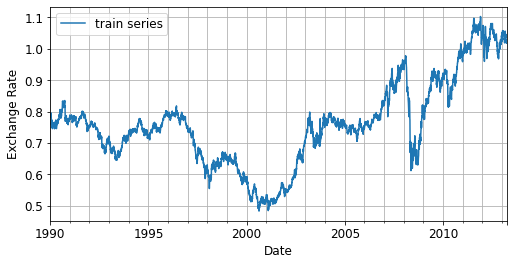
\includegraphics[width=\linewidth]{2_background/figures/exchange_rate_example.png}
            \caption{The exchange rate of two currencies between 1990 and 2013.}
    \endminipage\hfill
\end{figure}
\label{chicken}

\begin{figure}[htb]
    \centering
    \minipage{0.7\textwidth}
        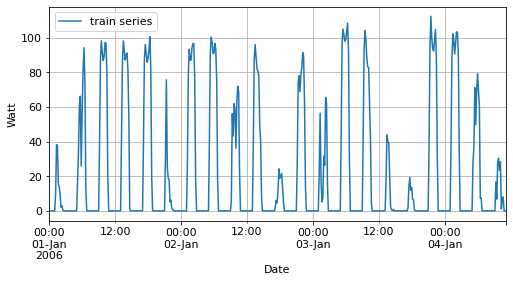
\includegraphics[width=\linewidth]{2_background/figures/solar_energy_zoomed_timeseries_3.png}
        \caption{First 500 datapoints of a timeseries in the solar-energy dataset.}
    \endminipage\hfill
\end{figure}
\label{fig:example_timeseries_solar_energy}

 Being able to interpret this data to predict future trends makes it possible to do preventive maintenance or make profitable investments. There are many methods of generating such predictions, ranging from simple heuristics to machine learning based methods. 


Before diving into different deep learning forecasting models in Section \ref{subsec:deep_learning_methods} it is important to understand how to quantify the accuracy of a forecasting model. Thus we will in \ref{subsec:error_metrics} present some commonly occurring methods for calculating errors of forecasts. In \ref{subsec:deep_learning_methods} we then present some information about how deep learning models are different from classical models as well as some of the benefits and drawbacks associated with deep learning algorithms.


\section{Time Series Forecasting}
\label{sec_time_series_forecasting}
Time series forecasting is the art of predicting future trends of time series based on past observations. It is a key technology within many fields and is fundamental to the business decision process for many companies. Time series forecasting differs from common machine learning tasks such as image recognition or language processing in that predictions are not binary. More specifically, in time series forecasting a prediction is expected to be a close estimate of future values. Thus, quantifying the magnitude of the error from the ground truth is of importance in order to properly evaluate the accuracy of a forecasting model. This is commonly done by calculating an error metric, the choice of which varies depending on what is being forecasted and on preference of the forecasting practitioner. In section \ref{subsec:error_metrics} some of these error metrics will be presented.

Timeseries forecasts often comes in one of two forms; probabilistic forecasts or point forecasts. A point forecast is a forecast which consist of only one estimation of the future values. This estimation could be either a single point in time or a series of points for several different timesteps. In figure \ref{fig:example_timeseries_forecast_point} an example of a point forecast for several timesteps can be seen. Point forecasts has the disadvantage that they do not confer how accurate they are which may lead to prectitioners being overly confident in the forecasts. This has caused several issues historically, non the least recently with covid-19 where rellying to heavily on point forecasts led to overly drastic measures for governments and hospitals \cite{IOANNIDIS2020}. Probabilistic forecasts such as the one in \ref{fig:example_timeseries_forecast_probabilistic} includes this information by generating prediction intervals of the forecasts.

\begin{figure}[htb]
    \centering
    \minipage{0.45\textwidth}
        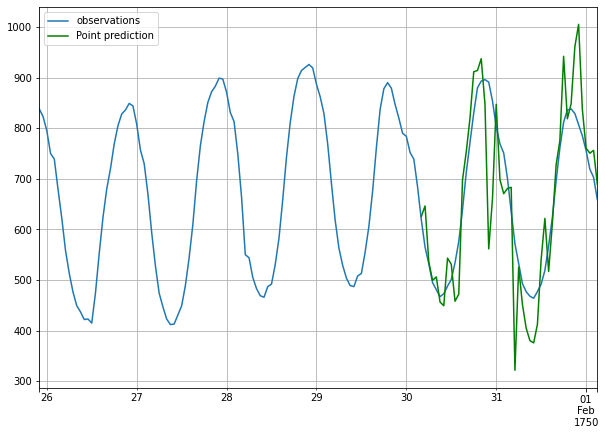
\includegraphics[width=\linewidth]{2_background/figures/timeseries_forecast_example_point.png}
        \caption{Time series point forecast}
        \label{fig:example_timeseries_forecast_point}
    \endminipage\hfill
    \minipage{0.45\textwidth}
        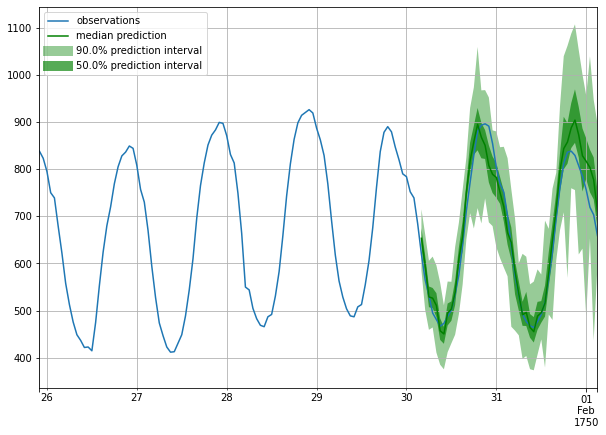
\includegraphics[width=\linewidth]{2_background/figures/timeseries_forecast_example_probability.png}
        \caption{Time series forecast with probability distribution}
        \label{fig:example_timeseries_forecast_probabilistic}
    \endminipage\hfill
\end{figure}
\label{fig:example_timeseries_forecast}

Many methods exist for generating forecasts on timeseries data, two common groups of these are machine learning based methods and trivial methods. A trivial forecasting method would be, for example, to predict that the next value should be the same as the last recently observed value or the average of the last N observations. For certain timeseries, trivial methods perform competitively and as such these are often held as a baseline to which new forecasting methods are being compared too. Some more complex methods include those based on regression analysis such as linear regression or autoregressive models such as ARIMA \cite{hyndman_forecasting_3rd}. Autoregressive models are a subset of regression models where the temporal ordering of the datapoints matter. I.e. autoregressive models use past observations to predict future values. 

Lately, inspired by the successful use of neural networks in other domains, several neural network based approaches for time series forecasting have been introduced. Early implementations such as simple multi-layered perceptrons did not perform competitively with the more classical approaches such ARIMA. However modern deep

Forecasting models for forecasting can also be split into further sub families such as whether they are local or global models. Local models are trained on individual time series while global models are trained on all time series in the training set. Essentially for a dataset with N timeseries, if using local models, one will have N different local models. If global models would be used only one model would be used for all N timeseries. Generally speaking, local models performs well for timeseries with much historical data. However for short or new timeseries, local models often perform poorly due to the inability to train the model on sufficiently large amounts of data points. This is known as the cold start problem. Since global models train on the entire dataset across all timeseries, any new timeseries added to the dataset suffer less from the cold start issue as the global model can use data from other timeseries as a basis for its predictions. \cite{wang_deep_2019} 



TODO

\begin{itemize}
\item Univariate (i.e. temperature over time) vs Multivariate (temperature, cloud coverage, wind, ..., over time) timeseries https://www.analyticsvidhya.com/blog/2018/09/multivariate-time-series-guide-forecasting-modeling-python-codes/
\item Point forecasts vs probabilistic forecasts
\end{itemize}


\section{Evaluating forecasting performance}
TODO
\begin{itemize}
\item Briefly explain backtesting
\item Explain k-fold validation with rolling datasets
\item Other methods for evaluating performance
\end{itemize}

\subsection{Error Metrics}
\label{subsec:error_metrics}
When a forecasting model generates predictions on a timeseries, one needs to be able to quantify the error of the prediction from true observed values. In order to do this many different error metrics exists each with its own benefits and drawbacks. Often the choice of metric is dependent on data, and business application where the prediction will be used. In this section some of the error metrics which are commonly occurring in literature are presented. These metrics are calculated automatically when performing a backtest in GluonTS, see \ref{subsec:gluonts_overview} for details about this process. Note that only a subset of the metrics available in GluonTS is presented here to form a basis for subsequent chapters.

\subsubsection{Absolute Error} 
The absolute error is calculated as the distance between the predicted value and the ground truth. An absolute error is positive and a value of 0 is optimal, i.e. the prediction fit perfectly. The absolute error is an intuitively simple error, thus it can easily be understood and discussed when comparing algorithms. 

However intuitive the absolute error is, there is a a key issue with this error and that is that it is scale dependent. I.e. the greater the values of the dataset being predicted on, the larger the absolute error will be. This makes it impossible to compare the accuracy of an algorithm across different datasets unless they have the same scale. \cite{hyndman_forecasting_nodate} Furthermore, scale dependent metrics such as these may not be suitable even for comparing between timeseries within a single dataset. Imagine a dataset such as the electricity dataset (see \ref{tab:datasets}) where each timeseries is the electricity consumption from a household. One household may contain many people and appliances while another may be a vacation home which is seldom visited. These two timeseries would have two different scales thus making it hard to compare the accuracy of the predictions using scale dependent metrics such as the absolute error. 

\subsubsection{Root Mean Squared Error - RMSE}
The root mean squared error is another scale dependent error such as the absolute error. RMSE is calculated by taking the square root of the mean of the squared error. TODO The RMSE thus punishes larger errors more than smaller errors due to it taking the power of the error before averaging. The RMSE is more complicated to interpret due to the non-linear nature, despite this, it is widely used in practise. \cite{hyndman_forecasting_nodate}.

\subsubsection{Mean Absolute Percentage Error - MAPE}
Percentage based errors such as the Mean Average Percentage Error normalizes the errors between 0 and 1 thus MAPE can be compared across datasets with different scales. While this is beneficial, MAPE suffer from other issues. For example MAPE becomes infinite or undefined if the ground truth is 0 for any parts of the prediction. Further issues exists for example that it penalizes negative errors more than positive errors. This has lead to variations of this metric to be created with their own pros and cons. \cite{hyndman_forecasting_nodate}

\subsubsection{Mean Average Scaled Error - MASE}
The MASE metric does not scale the errors based on the dataset used. Instead it scales the error on the error of a naive baseline forecasting model. An example of a baseline model could be one which predicts the future values to be the same as the last value. While this causes the MASE metric be scale independent MASE can still behave oddly in certain scenarios. For example if the  baseline model would perfectly predict a , this would cause the MASE to tend towards infinity. A MASE of 1 corresponds to that the algorithm under test is equally good as the naive model. A MASE below 1 means that the current model performs better than the naive model while a MASE above 1 means that the model performs worse than the naive baseline model. \cite{hyndman_forecasting_nodate}

\section{Deep Learning forecasting methods}
\label{subsec:deep_learning_methods}
Historically deep learning based methods for forecasting has been limited by the computational power available. Thus it is only recently that deep learning based methods has been used for forecasting.

\begin{itemize}
\item Benefits of deep learning
\item drawbacks of deep learning
\item Local versus global models(cold start)
\item common architectures (RNN(error accumulates when recursive strategy is used), LSTM, Fully connected, Hybrid approaches)
\end{itemize}
\subsection{Sources of randomness}
\begin{itemize}
\item Random initialization of weights
\item Random data shuffling
\item Random scheduling for multiprocessors, causing random data shuffling
\item Dropout
\end{itemize}
\subsection{Handling randomness}
\label{subsec:reproducibility}
\begin{itemize}
\item  Fixing the seed
\item Running on the same hardware
\item K-fold validation
\item Ensambles
\item Bagging
\end{itemize}
\subsection{Common approaches for ensuring reproducible results}
\begin{itemize}
\item everything in \ref{subsec:reproducibility}
\item public datasets
\item public code
\end{itemize}

\section{Related Work}
\label{subsec:related_work}
\subsection{Benchmarking}
\begin{itemize}
\item Why benchmarking
\item General info about benchmarking and how one would go ahead with benchmarking forecasting models.
\end{itemize}
\begin{itemize}
\item Specific difficulties with benchmarking deep learning models
\item Discussing some papers
\item Discussing another master thesis doing this
\end{itemize}

\subsubsection{Deep learning benchmarking suites}
\begin{itemize}
\item MLBench
\item MLPerf
\item DLBS
\end{itemize}

\subsubsection{Competitions}
\begin{itemize}
\item Basically present some info about the m competitions, what their purpose was. How they were implemented and why these are the closest thing available to a benchmarking suite. 
\end{itemize}
\begin{itemize}
\item Maybe briefly present what Kaggle offers.
\end{itemize}

\section{Gluon-TS}
\subsection{Overview}
\label{subsec:gluonts_overview}
Gluon-TS is an open source library which includes several deep learning algorithms, datasets and tools for building and evaluating deep learning based forecasting methods. In GluonTS, an \textit{Estimator} corresponds to the implementation of a forecasting method. An \textit{Estimator} can be trained on a dataset in order to generate a \textit{Predictor}. This \textit{Predictor} can then ingest timeseries in order to produce forecasts for the future values of the timeseries. 

In order to make it easy to evaluate the performance of an algorithm, GluonTS offers the \textit{backtest\_metrics} function. This function trains an \textit{Estimator} on a train dataset, the generated \textit{Predictor} is then used to generate predictions on a test dataset. Each of the timeseries in the test dataset will have the final N datapoints removed prior to passing them to the \textit{Predictor}.  The \textit{Predictor} then generates a prediction of length \textit{N} for each of the timeseries passed to it. Error metrics (see \ref{subsec:error_metrics}) are then calculated from the prediction and the datapoints which were removed earlier. In this example, \textit{N} corresponds to how many timesteps in the future one wishes to predict. 

GluonTS also contains Dockerfiles which makes it easy to create docker images with installations of GluonTS inside. These images are compatible with AWS SageMaker which allows them to be executed both in the cloud as well as locally. These images calls \textit{backtest\_metrics} when run and can thus be used to generate error metrics for any \textit{Estimator} class in GluonTS. 

\subsection{Algorithms}
GluonTS offers several forecasting models which can be used to generate predictions on timeseries data below I present most of these algorithms here. Only algorithms which were well documented in GluonTS \cite{gluonts-website} or which I could explain by sifting through the source code \cite{gluonts-github} are presented below.  

\subsubsection{CanonicalRNNEstimator}
This estimator is a bare bones recurrent neural network (RNN) estimator, with a single layer of LSTM cells \cite{gluonts-github}. LSTM stands for Long-Short-Term-Memory and is a cell architecture that allows RNNs to remember information from many timesteps back. An LSTM cell contains functionality which allows it to forget, ignore and store long term information. \cite{sherstinsky_fundamentals_2020}

\subsubsection{DeepFactorEstimator}
The DeepFactorEstimator is presented in \cite{wang_deep_2019} and consists of two main parts, a global and a local model. The global model is trained across all timeseries in order to capture complex non-linear patterns between the timeseries. The local model is meant to capture the local random effects of individual timeseries. This hybrid architecture is thus able to leverage the DNN capability of learning complex patterns as well as the computational efficiency of local models. In \cite{wang_deep_2019} three different versions of the DeepFactorEstimator is presented, the one implemented in GluonTS is the DF-RNN version. This version uses another RNN to model the local timeseries. The DF-RNN presented in the paper performs better than Prophet and MQ-RNN on the Electricity \ref{tab:datasets}, Taxi \ref{tab:datasets}, Traffic \ref{tab:datasets} and the Uber dataset both for short and long term forecasts. DeepAR however performed worse than DF-RNN on average but was more accurate on the short term forecasts for the Uber dataset. The Uber dataset is not available as part of GluonTS however it is mentioned here for completeness.

\subsubsection{DeepAR}  
\label{algo:deepar}
DeepAR presented in \cite{salinas_deepar_2019} is an RNN which produces probabilistic forecasts. The model learns a global representation across the timeseries and learns to identify seasonal behaviours in the data. DeepAR automatically adds certain meta information to the timeseries such as \textit{day-of-the-week}, \textit{hour-of-the-day}, \textit{week-of-the-year}, \textit{month-of-the-year}. Normally this type of meta information is added by the data scientist using the model, thus automating this procedure minimizes manual feature engineering. Another feature of DeepAR is the possibility to choose a likelihood distribution according to the data that it is to be trained on. In \cite{salinas_deepar_2019} the authors use two different distributions, the Gaussian Likelihood for real valued data and the negative binomial likelihood for postive count data. 
e
\subsubsection{DeepStateEstimator}
The DeepStateEstimator combines linear state space models for individual timeseries with a jointly learned RNN which is taught how to set the parameters for the linear state space models. This has the benefit that the labour intensive tuning of multiple state space models is done automatically by the RNN without sacrificing perfromance. This approach was shown to perform better than DeepAR \ref{algo:deepar} on the electricity dataset \ref{tab:datasets}. Additionally, it performed better than DeepAR on 4 out of 6 metrics on the traffic dataset \ref{tab:datasets}. Furthermore, this approach outperformed the ARIMA method and the ETS method on all the datasets \ref{rangapuram_deep_2018}. 

\subsubsection{GaussianProcessEstimator}
The GaussianProcessEstimator is a local model where each timeseries in the dataset is modeled by a single gaussian process. The gaussian process takes a kernel to use for the gaussian processes as a parameter. 
\cite{gluonts-website}

\subsubsection{GPVAREstimator and DeepVAREstimator}
\label{algo:gpvar}
The GPVAREstimator was presented as GP-Copula in this paper \cite{salinas_high-dimensional_2019}. It is a RNN model for handling multivariate timeseries which uses a gaussian copula technique for automatic data transformation and scaling . Further, a dimensionality reduction technique is employed which minimizes the parameters needed to calculate a covariance matrix from \textit{O($n^2$)} to \textit{O(n)}. This allows for much larger multivariate timeseries datasets. In \cite{salinas_high-dimensional_2019} the authors evaluated the GPVAREstimator on six datasets, all available in GluonTS see \ref{ds:nips} \& \ref{tab:datasets}. Additionally, the GPVAREstimator was compared against other multivariate forecasting algorithms, amongst which one was a version of the DeepAREstimator \ref{algo:deepar} which was altered to handle multivariate timeseries. In in GluonTS this algorithm is named DeepVAREstimator and was in the paper referred to as \textit{vec-LSTM}. 

\subsubsection{LSTNetEstimator}
The LSTNetEstimator can be seen as a hybrid approach where long term patterns of the data is captured by a neural network architecture, these long term patterns are combined with a classical autoregressive model when generating predictions. The neural network architecture consists of four parts, a CNN, a RNN a novel RNN-skip layer and a fully connected layer. The RNN-skip layer makes up for the incapability of the LSTM cells in a RNN to remember very long term information by only updating the cells periodically \cite{lai_modeling_2018}.

\subsubsection{NBEATSEstimator and NBEATSEnsembleEstimator}
In \cite{oreshkin_n-beats_2020} a univariate deep learning model for forecasting named N-BEATS is presented. The authors of N-BEATS expressed that their goal with this algorithm was disprove the notion that deep learning models had inferior performance  compared to classical models. The authors reported a higher accuracy with the N-BEATS model over all the models it was compared to. 

The N-BEATS algorithm is an ensemble of multiple smaller algorithms which are all trained with different goals in mind. In \cite{oreshkin_n-beats_2020} the ensemble consists of 180 smaller algorithms. These were optimized for different metrics (MASE, sMASE, MAPE etc.) and six different context lengths. Furthermore, bagging was used by running multiple runs of the algorithms with random initializations of the networks. A prediction of the N-BEATS model is the median value of the predictions of the algorithms in the ensemble. 

A high level overview of the structure of each of the models in the ensemble is that each consists of multiple fully connected layers chained together to form blocks of networks. Each block in turn is chained together in order to form a stack. These stacks are also chained in order to form the final network. Thus this is a nested architecture consisting of fully connected layers.

GluonTS implements the N-BEATS model as the NBEATSEnsambleEstimator and the smaller algorithms in the ensemble as the NBEATSEstimator. There are some differences between the implementation in \cite{oreshkin_n-beats_2020} and that of GluonTS. Specifically, the training data is sampled differently in GluonTS than in the paper \cite{gluonts-website}. 

\subsubsection{Naive2Predictor}
the Naive2Predictor is a GluonTS implementation of the Naïve 2 forecasting method used as a reference in the m4 competition \cite{makridakis_m4_2020}. The Naive2Predictor predicts the future values to be that of the last datapoint in the timeseries adjusted by some seasonality. In GluonTS this seasonality can be deduced from the frequency of the data used or by passing a custom seasonality via the \textit{season\_length} parameter \cite{gluonts-website}. 

\subsubsection{NPTSPredictor}
The NPTSPredictor predicts future values by sampling from previous data in the timeseries. The way that the samples are selected from the previous data can be modified via the hyperparameters. One can sample uniformly across all previous values in the timeseries. One can also bias the sampling to more often sample from more recent datapoints by choosing an exponential kernel. Additionally it is possible to only sample values from seasonal values \cite{gluonts-website}.

\subsubsection{ProphetPredictor}
Prophet is a nonlinear regression model developed at Facebook which frames the timeseries forecasting problem as a curve fitting exercise \cite{hyndman_forecasting_3rd}. This is different from many other forecasting models for timeseries which leverage the temporal aspect of timeseries when forecasting. Prophet was created with three goals in mind; it should be easy to use for people without  much knowledge about timeseries methods, it should work for many different forecasting tasks which may have distinct features. Finally it should contain logic which makes it easy to identify how good the generated forecasts of Prophet are \cite{taylor_forecasting_2017}. 

\subsubsection{RForecastPredictor}
The RForecastPredictor is a wrapper which allows a user of GluonTS to use the popular forecasting package \textit{forecast} inside of GluonTS.  The forecaster to use inside of the R package can be selected by passing the name of the method as a hyperparameter\cite{gluonts-website,r-forecast-package}.

\subsubsection{SeasonalNaivePredictor}
The SeasonalNaivePredictor is a naive model which predicts the future value to be the same as the value of the previous season. This is a very simple model however an example explains its functionality best. If I want to use the SeasonalNaivePredictor to forecast the average temperature of June. The SeasonalNaivePredictor will return the average temperature for last year in June. In GluonTS, if not enough data exists (i.e. no data for last year in June) the mean of all the data is returned\cite{gluonts-website,hyndman_forecasting_3rd}

\subsubsection{MQCNNEstimator, MQRNNEstimator}
The GluonTS seq2seq package contains two forecasting algorithms, MQ-CNN and MQ-RNN, as presented in \cite{wen_multi-horizon_2018} as two implementations of their proposed MQ framework. The MQ framework is based on the Seq2Seq architecture\cite{seq2seq} which consists of an encoder and a decoder network. A Seq2Seq architecture encodes the training data into a hidden state which the decoder network then decompresses. Normally in Seq2Seq architectures, the RNN models tend to accumulate errors as the forecasts of an RNN for a timepoint \textit{t} will be reused in order to generate a forecast for time \textit{t+1}. By instead training the model to generate multiple point forecast for each timepoint in the horizon one wishes to forecast on, the errors tend to grow smaller. This is called \textit{Direct Multi-Horizon Forecasting} and it is one of the changes introduced in the MQ framework. Further, the MQ framework allows for different encoders to used. Two of these are implemented in GluonTS, one with a CNN and one with a RNN. These are the MQCNNEstimator and the MQRNNEstimator respectively \cite{gluonts-website}.

\subsubsection{SimpleFeedForwardEstimator}
The SimpleFeedForwardEstimator in GluonTS is a traditional Multi Layer Perceptron (MLP) which can be dynamically resized based on user parameters. Per default it has two densely connected layers with 40 nodes in the input layer and 40 times the prediction length number of cells in the hidden layer. Furthermore it has an added layer for performing probability based predictions instead of only point predictions. This layer consists of a number of sublayers equal to the desired prediction length. Each of these layers consists of 40 nodes (i.e. the size of the output layer). After each hidden layer an optional batch normalization layer can be attached \cite{gluonts-github}.

\subsubsection{TransformerEstimator}
The transformer estimator is a sequence to sequence model which replaces the classical RNN encoder and decoders with more parallelizable NN components. A RNN requires data to passed sequentially in order to learn dependencies between datapoints. This introduces a bottleneck and makes RNNs harder to train efficiently on modern hardware accelerators such as GPUs. The Transformer architecture presented in \cite{vaswani_attention_nodate} alliviates this by leveraging parallelizable architectures such as feed forward networks as well as making heavy use of attention. Attention means that the architecture automatically can identify which parts of the input data is most relevant to the value we are trying to predict\cite{vaswani_attention_nodate}. I.e. for the next value we are predicting, the most relevant previous values may be any or all of the previous \textit{n} observations.  In GluonTS the Transformer is implemented under as the TransformerEstimator. \cite{gluonts-website}

\subsubsection{Wavenet}
Based on the PixelCNN algorithm. Wavenet synthesizes speech on the waveform layer. 
Wavenet has many techniques allowing for extremely deep networks without unreasonable execution overhead. 

\subsection{Datasets}
GluonTS offers 17 datasets ready to be used for training and evaluation, in table \ref{tab:datasets} these are presented.

\begin{table}[ht]
    \centering
    \begin{tabular}{p{0.23\linewidth} | p{0.09\linewidth} | p{0.68\linewidth}}
        Name & Freq & Description \\ \hline
        Electricity & Hourly & Hourly electricity consumption of 370 clients sampled between 2011 - 2014. The original dataset on UCL was sampled each 15 minutes whilst the dataset in GluonTS had the data resampled into hourly series \cite{gluonts-website, salinas_high-dimensional_2019}.\\
        \hline
        Exchange Rate & B & Daily currency exchange rates of eight countries; Australia, Britain, Canada, China, Japan, New Zealand, Singapore and Switzerland between 1990 and 2016  \cite{lai_modeling_2018}. \\
        \hline
        Traffic & H & This dataset contains the hourly occupancy rate of 963 car lanes of the San Francisco Bay are freeways \cite{gluonts-github}. \\
        \hline
        Solar Energy & 10 Min & The solar power production records in the year of 2006, sampled every 10 minutes from 137 solar energy plants in Alabama \cite{lai_modeling_2018}. \\
        \hline
        Electricity NIPS & H & The Electricity dataset with additional processing \cite{salinas_high-dimensional_2019}. \\
        \hline
        Exchange Rate NIPS & B & The Exchange Rate dataset with additional processing \cite{salinas_high-dimensional_2019}. \\
        \hline
        Solar Energy NIPS & H & The Solar Energy dataset with additional processing \cite{salinas_high-dimensional_2019}. \\
        \hline
        Traffic NIPS & H & The Traffic dataset with additional processing \cite{salinas_high-dimensional_2019}. \\
        \hline
        Wiki Rolling NIPS & D & The Wiki dataset contains the amount of daily views for 2000 pages on Wikipedia \cite{salinas_high-dimensional_2019}. \\
        \hline
        Taxi & 30 Min & Number of taxi rides taken on 1214 locations in New York city every 30 minutes in the month of January 2015. The test set is sampled on January 2016 \cite{salinas_high-dimensional_2019}.  \\
        \hline
        M4 Hourly & H & Hourly timeseries used in the M4 competition randomly sampled from the ForeDeCk database \cite{makridakis_m4_2020}.\\
        \hline
        M4 Daily & D & Daily timeseries used in the M4 competition randomly sampled from the ForeDeCk database \cite{makridakis_m4_2020}.\\
        \hline
        M4 Weekly & W & Weekly timeseries used in the M4 competition randomly sampled from the ForeDeCk database \cite{makridakis_m4_2020}.\\
        \hline
        M4 Monthly & M & Monthly timeseries used in the M4 competition randomly sampled from the ForeDeCk database \cite{makridakis_m4_2020}.\\
        \hline
        M4 Quarterly & 3M & Quarterly timeseries used in the M4 competition randomly sampled from the ForeDeCk database \cite{makridakis_m4_2020}.\\
        \hline
        M4 Yearly & Y & Yearly timeseries used in the M4 competition randomly sampled from the ForeDeCk database \cite{makridakis_m4_2020}.\\
        \hline
        M5 Dataset & D & Daily Walmart sales for 3049 products across 10 stores \cite{gluonts-github, m5}. 
    \end{tabular}
    \caption{Datasets available in GluonTS.}
    \label{tab:datasets}
\end{table}

\section{Runtool}
\label{subsec:runtool}
\subsection{Config files}
\subsection{Defining experiments}

\section{Statistical tests for distributions}
\subsection{T-test}
\label{subsubsec:t-test}
TODO present t test briefly
\subsection{Welch's T-Test}
\label{subsubsec:welchs-t-test}
TODO present Welchs T-test briefly
\subsection{Kolmogorov-Smirnov Test}
\label{subsubsec:ks-test}
TODO present ks test
\subsection{Continous Kolmogorov-Smirnov test}
\label{subsubsec:cont-ks-test}
TODO this is more of an optimization as the ks-test seem to work just fine
\subsection{Dvoretzky–Kiefer–Wolfowitz inequality}
\label{subsubsec:dvoretzky-kiefer-wolfowitz}
This will probs be discussed as part of KS test instead

\section{Dataset characteristics}
\label{sec:dataset_characteristics}
\subsection{STL - decomposition}
\subsection{Seasonality}
\subsection{Trend}
\subsection{Stationarity}


% ---------------------------------------------------------------------------
% ----------------------- end of thesis sub-document ------------------------
% ---------------------------------------------------------------------------